
\begin{center}
\Huge
Tangentplaner og gradientvektorer
\end{center}

\section*{Partielle afledede}
\stepcounter{section}

Lad os sige, at vi har et punkt $P(x_0,y_0,f(x_0,y_0))$. Til en funktion $f$ af to variable, så vil grafen for $f$ - hvis den er pæn nok - have en plan i punktet $P(x_0,y_0,f(x_0,y_0))$, der rører grafen for $f$ i netop det punkt og i en omegn af punktet ikke rører andre punkter. Denne plan kaldes for \textit{tangentplanen} for $f$ i punktet $P(x_0,y_0,f(x_0,y_0))$. 

\begin{setn}[Tangentplan]
	Lad $f:\mathbb{R}^2 \to \mathbb{R}$ samt et punkt $P(x_0,y_0,f(x_0,y_0))$ være givet. 
	Så er tangentplanen til $f$ i $P$ givet ved ligningen
	\begin{align}\label{eq:tangentplan}
		z = f(x_0,y_0) + f_x'(x_0,y_0)(x-x_0) + f_y'(x_0,y_0)(y-y_0).
	\end{align}
\end{setn}
Vi vil ikke bevise denne sætning. 

\begin{exa}
	Lad $f$ være givet ved
	\begin{align*}
		f(x,y) = x^2+y^2.
	\end{align*}
	Så bestemmer vi tangentplanen for $f$ i $(2,3,f(2,3))$ på følgende vis: Vi bestemmer først
	$f(2,3)$:
	\begin{align*}
		f(2,3) = 4+9=13.
	\end{align*}
	Vi bestemmer de partielle afledede:
	\begin{align*}
		&f_x'(x,y) =2x \ \Rightarrow \ f_x'(2,3) = 4, \\
		&f_y'(x,y) =2y \ \Rightarrow \ f_y'(2,3) = 6.
	\end{align*}
	Vi indsætter nu i formlen \eqref{eq:tangentplan}:
	\begin{align*}
		z &= f(2,3) + f_x'(2,3)(x-2) + f_y'(x_0,y_0)(y-3)(\\
		&= 13+4(x-2) + 6(y-3),
	\end{align*}
	hvilket er ligningen for tangentplanen. Dette kan også ses af Fig. \ref{fig:tangentplan}
	\begin{figure}[H]
		\centering
		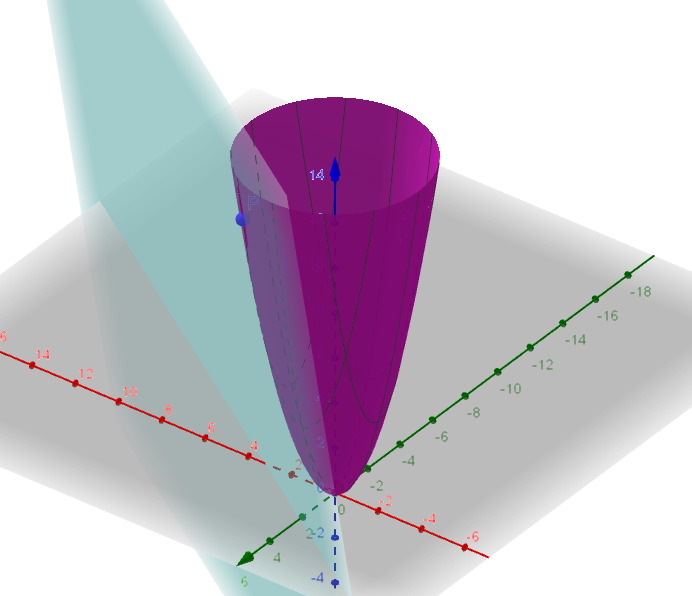
\includegraphics[width = 0.5\textwidth]{Billeder/tangentplan.png}
		\caption{Tangentplan i $(2,3,f(2,3))$.}
		\label{fig:tangentplan}
	\end{figure}
\end{exa}

\section*{Opgave 1}
\begin{enumerate}[label=\roman*)]
	\item Lad $f$ være givet ved
	\begin{align*}
		f(x,y) = x^3-y^2.
	\end{align*}
	Bestem en ligning for tangentplanen i punkterne $(-1,3,f(-1,3))$ og $(2,4,f(2,4))$.
	\item Lad $f$ være givet ved
	\begin{align*}
		f(x,y) = xy+\cos(xy^2).
	\end{align*}
	Bestem en ligning for tangentplanen i punktet $(\pi,\frac{\pi}{4},f(\pi,\frac{\pi}{4}))$.
	\item Lad $f$ være givet ved
	\begin{align*}
		f(x,y) = \sqrt{x+y}.
	\end{align*}
	Bestem en ligning for tangentplanen i punktet $(12,4,f(12,4))$. 
	\item Lad $f$ være givet ved 
	\begin{align*}
		f(x,y) = (x+2y)^3
	\end{align*}
	Bestem en ligning for tangentplanen i punktet $(3,6,f(3,6))$.
\end{enumerate}

\section*{Opgave 2}
Vi husker på, at ligningen for planen $L$ er givet ved
\begin{align*}
	a(x-x_0)+b(y-y_0)+c(x-x_0)=0,
\end{align*}
hvor $\vv{n}$ givet ved
\begin{align*}
	\vv{n} = 
	\begin{pmatrix}
		a \\ b \\ c
	\end{pmatrix}
\end{align*}
er en normalvektor for $L$. 
\begin{enumerate}[label=\roman*)]
	\item Brug ligningen for tangentplanen til at argumentere for, at vektoren $\vv{v}$ givet 
	ved
	\begin{align*}
		\vv{v} = 
		\begin{pmatrix}
			f_x'(x_0,y_0) \\
			f_y'(x_0,y_0) \\
			-1
		\end{pmatrix}
	\end{align*}
	må være en normalvektor til tangentplanen. 
\end{enumerate}
\section*{Opgave 3 (Lidt svær)}

\begin{enumerate}[label=\roman*)]
	\item Argumentér for, at vektoren $\vv{v_x}$ givet ved 
	\begin{align*}
		\vv{v_x} = 
		\begin{pmatrix}
			1 \\ 0 \\ f_x'(x_0,y_0)
		\end{pmatrix}
	\end{align*}
	er retningsvektor for tangentlinjen for snitkurven gennem $(x_0,y_0)$ langs $y$-planen. 
	\item Argumentér for, at vektoren $\vv{v_y}$ givet ved 
	\begin{align*}
		\vv{v_y} = 
		\begin{pmatrix}
			0 \\ 1 \\ f_y'(x_0,y_0)
		\end{pmatrix}
	\end{align*}
	er retningsvektor for tangentlinjen for snitkurven gennem $(x_0,y_0)$ langs $x$-planen. 
	\item Brug dette til at argumentere for, at vektorerne $\vv{v_x}$ og $\vv{v_y}$ ligger i 
	tangentplanen. 
	\item Krydsproduktet mellem to vektorer $\vv{a}$ og $\vv{b}$ i rummet er givet ved
	\begin{align*}
		\begin{pmatrix}
			a_1 \\ a_2 \\ a_3
		\end{pmatrix} \times 
		\begin{pmatrix}
			b_1 \\ b_2 \\ b_3
		\end{pmatrix} = 
		\begin{pmatrix}
		a_2b_3-a_3b_2 \\ 
		-a_1b_3+a_3b_1 \\
		a_1b_2-a_2b_1
		\end{pmatrix}
	\end{align*}
	og krydsproduktet giver en vektor, der er orthogonal på både $\vv{a}$ og $\vv{b}$. 
	Brug dette til at argumentere for, at vektoren
	\begin{align*}
		\begin{pmatrix}
			f_x'(x_0,y_0) \\
			f_y'(x_0,y_0) \\
			-1
		\end{pmatrix}
	\end{align*}
	er en normalvektor til tangentplanen i $(x_0,y_0,f(x_0,y_0))$.
	\item Brug dette samt planens ligning til at bevise Sætning 1.1
\end{enumerate}
\section*{Opgave 4}
Aflevering